\chapter{欧氏空间中的曲线坐标与张量指标}

\section{曲线坐标与自然基底}

在三维欧氏空间 $\mathbb{R}^{3}$ 中, 笛卡尔坐标 $(x,y,z)$ 是最常用的坐标系. 然而, 许多物理问题本身具有柱对称、球对称或其他几何结构, 此时采用与几何结构相适应的曲线坐标, 往往能使问题的表达更加简洁. 

设一组曲线坐标为
\[
(q^{1},q^{2},q^{3}).
\]
空间中一点的位置矢量可看作这些坐标的函数: 
\[
\bm{r}=\bm{r}(q^{1},q^{2},q^{3}).
\]
需要注意的是, $q^{i}$ 是描述空间点的坐标参数, 而不是位置矢量 $\bm{r}$ 在某组基底下的分量. 因此, 在一般曲线坐标中, 不能将位置矢量写成
\[
\bm{r}=q^{i}\bm{e}_{i}.
\]
\begin{figure}[h]
	\centering
	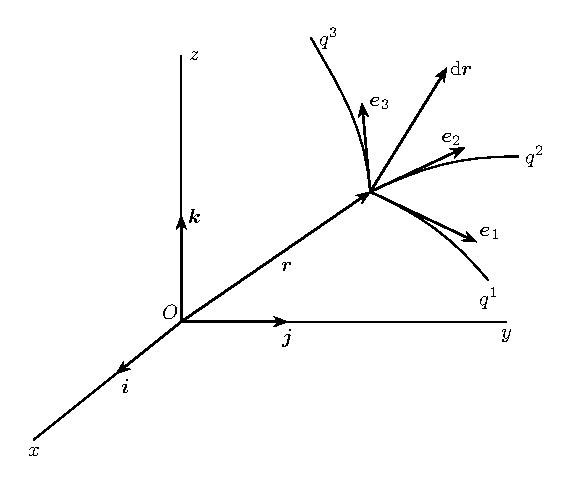
\includegraphics[width=0.5\linewidth]{figure/fig1.1}
	\caption[曲线坐标系]{曲线坐标系}
	\label{fig:1.1}
\end{figure}

例如, 在柱坐标 $(\rho,\varphi,z)$ 中, 
\[
\bm{r}
=
\rho\cos{\varphi}\,\bm{i}
+
\rho\sin{\varphi}\,\bm{j}
+
z\bm{k},
\]
但不能写成
\[
\bm{r}
=
\rho\bm{e}_{\rho}
+
\varphi\bm{e}_{\varphi}
+
z\bm{e}_{z}.
\]
其原因在于 $\varphi$ 是角坐标, 并不是沿 $\bm{e}_{\varphi}$ 方向的长度分量. 
\begin{figure}[h]
	\centering
	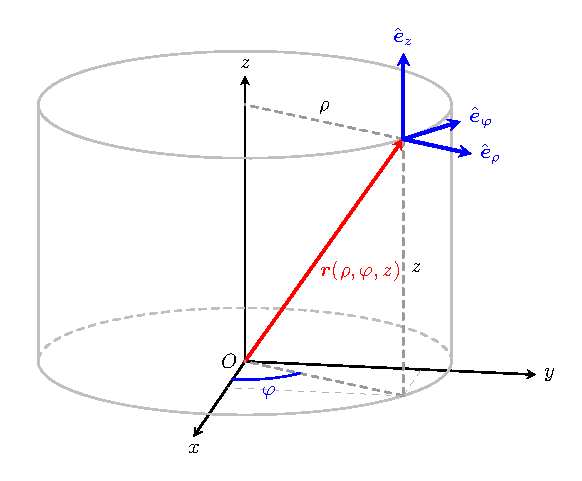
\includegraphics[width=0.5\linewidth]{figure/fig1.2}
	\caption[柱坐标系]{柱坐标系}
	\label{fig:1.2}
\end{figure}

曲线坐标的自然协变基底定义为
\begin{equation}
\bm{e}_{i}
=
\frac{\partial \bm{r}}{\partial q^{i}},
\qquad i=1,2,3. \label{eq:1.1}
\end{equation}
从几何上看, $\bm{e}_{i}$ 给出了只改变坐标 $q^{i}$ 时位置矢量的变化方向. 由于曲线坐标的坐标线一般不是直线, $\bm{e}_{i}$ 通常随空间位置而变化. 

当坐标 $q^{i}$ 改变一个无穷小量 $\dif q^{i}$ 时, 由\eqref{eq:1.1}可得位移矢量
\[
\dif\bm{r}
=
\frac{\partial \bm{r}}{\partial q^{i}}\dif q^{i}
=
\bm{e}_{i} \dif q^{i}.
\]
以下采用爱因斯坦求和约定: 重复出现的一上一下指标默认求和. 

\section{协变基底与逆变基底}

在一般曲线坐标中, 基底 $\bm{e}_{i}$ 未必正交, 也未必归一. 仅用这一组基底处理向量分量并不总是方便, 因此需要引入与 $\bm{e}_{i}$ 对偶的逆变基底 $\bm{e}^{i}$, 使其满足
\begin{equation}
\bm{e}_{i}\cdot \bm{e}^{j}
=
\delta_{i}^{j}. \label{eq:1.2}
\end{equation}
其中 $\delta_{i}^{j}$ 是 Kronecker 符号: 
\[
\delta_{i}^{j}=
\begin{cases}
1,& i=j,\\
0,& i\neq j.
\end{cases}
\]
在欧氏空间的曲线坐标中, 逆变基底可以写成坐标函数的梯度: 
\[
\bm{e}^{i}=\nabla q^{i}.
\]
这是因为
\[
\bm{e}_{i}\cdot \bm{e}^{j}
=
\frac{\partial \bm{r}}{\partial q^{i}}\cdot \nabla q^{j}
=
\frac{\partial q^{j}}{\partial q^{i}}
=
\delta_{i}^{j}.
\]
对任意向量 $\bm{A}$, 可以用两套基底展开: 
\[
\bm{A}
=
A^{i}\bm{e}_{i}
=
A_{i}\bm{e}^{i}.
\]
其中 $A^{i}$ 称为逆变分量, $A_{i}$ 称为协变分量. 这里应当区分坐标参数与向量分量: $q^{i}$ 描述空间点的位置, 而 $A^{i}$ 描述向量 $\bm{A}$ 在协变基底 $\bm{e}_{i}$ 下的展开系数. 在一般曲线坐标中, 这两类量并不具有相同的几何意义. 

\section{度规张量与线元}

曲线坐标中基底的长度和夹角由度规张量描述. 协变度规定义为
\begin{equation}
g_{ij}
=
\bm{e}_{i}\cdot \bm{e}_{j}. \label{eq:1.3}
\end{equation}
逆变度规定义为
\[
g^{ij}
=
\bm{e}^{i}\cdot \bm{e}^{j}.
\]
矩阵意义下, $(g^{ij})$ 是 $(g_{ij})$ 的逆矩阵, 即
\[
g^{ik}g_{kj}
=
\delta^{i}_{j}.
\]
由位移公式 $\dif\bm{r}=\bm{e}_{i} \dif q^{i}$ 及\eqref{eq:1.3}, 得到线元平方: 
\begin{equation}
\dif s^{2}
=
\dif\bm{r}\cdot \dif\bm{r}
=
g_{ij}\dif q^{i} \dif q^{j}. \label{eq:1.4}
\end{equation}
因此, 度规张量给出了坐标微分 $\dif q^{i}$ 与实际几何长度之间的关系. 

度规还负责升降指标. 若
\[
\bm{A}=A^{i}\bm{e}_{i}=A_{i}\bm{e}^{i},
\]
则有
\[
A_{i}=g_{ij}A^{j},
\]
以及
\[
A^{i}=g^{ij}A_{j}.
\]
内积可以写成
\begin{equation}
\bm{A}\cdot \bm{B}
=
g_{ij}A^{i}B^{j}
=
A^{i}B_{i}
=
A_{i}B^{i}. \label{eq:1.5}
\end{equation}
在笛卡尔正交归一坐标中, 
\[
g_{ij}=\delta_{ij},
\qquad
g^{ij}=\delta^{ij},
\]
此时协变分量和逆变分量可以不加区分. 对于一般曲线坐标, 这种简化通常不再成立. 

\section{体积元与 Levi-Civita 张量}

记度规矩阵的行列式为
\[
g=\det{(g_{ij})}.
\]
在曲线坐标中, 三维体积元为
\begin{equation}
\dif V
=
\sqrt{g}\,\dif q^{1}\dif q^{2}\dif q^{3}. \label{eq:1.6}
\end{equation}
其中 $\sqrt{g}$ 是坐标体积元相对于欧氏几何体积元的伸缩因子. 

为了描述叉积、体积取向和旋度, 需要引入 Levi-Civita 对象. 先定义排列符号 $[ijk]$: 
\[
[123]=1,
\]
交换任意两个指标变号, 若有重复指标则为 $0$. 

排列符号 $[ijk]$ 本身不是张量. 在曲线坐标中, Levi-Civita 张量定义为
\begin{equation}
\varepsilon_{ijk}
=
\sqrt{g}\,[ijk],
\qquad
\varepsilon^{ijk}
=
\frac{1}{\sqrt{g}}[ijk]. \label{eq:1.7}
\end{equation}
于是有
\[
\varepsilon_{123}=\sqrt{g},
\qquad
\varepsilon^{123}=\frac{1}{\sqrt{g}}.
\]
在笛卡尔正交归一坐标中, $g=1$, Levi-Civita 张量退化为普通排列符号. 

Levi-Civita 张量不仅依赖维数, 还依赖空间的取向和度规结构. 没有度规, 就不能自然地定义升降指标; 没有取向, 就不能区分正负体积元. 

\section{向量代数的指标写法}

在三维有向欧氏空间中, 常见的向量运算可以用度规和 Levi-Civita 张量统一表示. 

设
\[
\bm{A}=A^{i}\bm{e}_{i},
\qquad
\bm{B}=B^{j}\bm{e}_{j}.
\]
内积已由\eqref{eq:1.5}给出. 叉积依赖三维空间的度规和取向, 基底之间满足
\[
\bm{e}_{i}\times \bm{e}_{j}
=
\varepsilon_{ijk}\bm{e}^{k}.
\]
因此
\begin{equation}
\bm{A}\times \bm{B}
=
A^{i}B^{j}(\bm{e}_{i}\times \bm{e}_{j})
=
\varepsilon_{ijk}A^{i}B^{j}\bm{e}^{k}. \label{eq:1.8}
\end{equation}
如果希望写成协变基底 $\bm{e}_{k}$ 的展开形式, 可以利用
\[
\bm{e}^{k}=g^{k\ell}\bm{e}_{\ell},
\]
于是
\[
\bm{A}\times \bm{B}
=
g^{k\ell}\varepsilon_{ijk}A^{i}B^{j}\bm{e}_{\ell}.
\]
因此叉积的逆变分量为
\begin{equation}
(\bm{A}\times \bm{B})^{\ell}
=
g^{k\ell}\varepsilon_{ijk}A^{i}B^{j}
=
\varepsilon^{\ell}{}_{ij}A^{i}B^{j}. \label{eq:1.9}
\end{equation}
三重混合积为
\[
\bm{A}\cdot(\bm{B}\times \bm{C})
=
\varepsilon_{ijk}A^{i}B^{j}C^{k},
\]
该式表示由三个向量张成的有向体积. 

在笛卡尔正交归一坐标中, $\varepsilon_{ijk}=[ijk]$, 于是熟悉的公式恢复为
\[
\bm{A}\cdot(\bm{B}\times \bm{C})
=
[ijk]A^{i}B^{j}C^{k}.
\]

\begin{example}{用指标形式计算叉积}{1,1}
设在一般曲线坐标中 $\bm{A}=A^{i}\bm{e}_{i}$, $\bm{B}=B^{j}\bm{e}_{j}$. 证明叉积的逆变分量可以写成
\[
(\bm{A}\times\bm{B})^{\ell}
=
g^{k\ell}\varepsilon_{ijk}A^{i}B^{j}.
\]
\end{example}

\begin{solution}
由自然基底叉积 $\bm{e}_{i}\times\bm{e}_{j} = \varepsilon_{ijk}\bm{e}^{k}$, 以及\eqref{eq:1.8}, 有
\[
\bm{A}\times\bm{B}
=
A^{i}B^{j}\varepsilon_{ijk}\bm{e}^{k}.
\]
利用 $\bm{e}^{k}=g^{k\ell}\bm{e}_{\ell}$, 得到
\[
\bm{A}\times\bm{B}
=
g^{k\ell}\varepsilon_{ijk}A^{i}B^{j}\bm{e}_{\ell},
\]
与 $\bm{A}\times\bm{B}=(\bm{A}\times\bm{B})^{\ell}\bm{e}_{\ell}$ 比较, 即得所证. 由此可见, 叉积不仅依赖排列的反对称性, 还依赖度规和空间取向. 
\end{solution}

\section{梯度、散度、旋度与拉普拉斯算子}

曲线坐标中的微分算符不能简单照搬笛卡尔形式, 因为基底本身依赖坐标. 

\subsection{梯度}

设 $f$ 为标量场, 其微分为
\[
\dif f
=
\partial_{i} f\,\dif q^{i}.
\]
梯度向量由下式定义: 
\[
\dif f
=
\nabla f\cdot \dif\bm{r}.
\]
由于 $\dif\bm{r}=\bm{e}_{i} \dif q^{i}$, 若将梯度写为 $\nabla f=(\nabla f)^{i}\bm{e}_{i}$, 则
\[
\nabla f\cdot \dif\bm{r}
=
g_{ij}(\nabla f)^{i} \dif q^{j}.
\]
与 $\dif f=\partial_{j} f\,\dif q^{j}$ 比较, 可得
\[
g_{ij}(\nabla f)^{i}=\partial_{j} f.
\]
因此
\[
(\nabla f)^{i}
=
g^{ij}\partial_{j} f.
\]
因此梯度可写为
\begin{equation}
\nabla f
=
g^{ij}\partial_{j} f\,\bm{e}_{i}
=
(\partial_{i} f)\bm{e}^{i}. \label{eq:1.10}
\end{equation}

\subsection{散度}

设向量场为 $\bm{A}=A^{i}\bm{e}_{i}$. 在一般曲线坐标中, 散度不能简单写成 $\partial_{i} A^{i}$, 而应写为
\begin{equation}
\nabla\cdot\bm{A}
=
\frac{1}{\sqrt{g}}\partial_{i}(\sqrt{g}\,A^{i}). \label{eq:1.11}
\end{equation}
这一表达式可理解为通量密度的局部变化率, 其中因子 $\sqrt{g}$ 来自曲线坐标中的体积元. 

在笛卡尔正交归一坐标中, $\sqrt{g}=1$, 上式退化为
\[
\nabla\cdot\bm{A}
=
\partial_{i} A^{i}.
\]

\subsection{旋度}

设向量场 $\bm{A}=A^{i}\bm{e}_{i}$, 其对应的一形式分量为 $A_{i}=g_{ij}A^{j}$. 旋度的逆变分量为
\begin{equation}
(\nabla\times\bm{A})^{i}
=
\varepsilon^{ijk}\partial_{j} A_{k}. \label{eq:1.12}
\end{equation}
其中 $A_{k}$ 是协变分量, 而不是正交单位基底下的物理分量. 因此
\[
\nabla\times\bm{A}
=
\varepsilon^{ijk}\partial_{j} A_{k}\,\bm{e}_{i}.
\]
由于 Levi-Civita 张量反对称, 协变导数中的对称联络项在反对称化中抵消, 因此上述公式可以用普通偏导表示. 

\subsection{拉普拉斯算子}

标量场 $f$ 的拉普拉斯算子定义为 $\nabla^{2} f = \nabla\cdot(\nabla f)$. 结合梯度公式\eqref{eq:1.10}与散度公式\eqref{eq:1.11}, 得到
\begin{equation}
\nabla^{2} f
=
\frac{1}{\sqrt{g}}
\partial_{i}
\left(
\sqrt{g}\,g^{ij}\partial_{j} f
\right). \label{eq:1.13}
\end{equation}
这就是欧氏空间曲线坐标中的 Laplace-Beltrami 形式. 

在笛卡尔正交归一坐标中, 
\[
g^{ij}=\delta^{ij},
\qquad
\sqrt{g}=1,
\]
于是有
\[
\nabla^{2} f
=
\partial_{i}\partial_{i} f.
\]

\section{正交曲线坐标与物理分量}

若曲线坐标是正交的, 则当 $i\neq j$ 时有 $g_{ij}=0$. 此时线元可以写成
\begin{equation}
\dif s^{2}
=
h_{1}^{2}(\dif q^{1})^{2}
+
h_{2}^{2}(\dif q^{2})^{2}
+
h_{3}^{2}(\dif q^{3})^{2}, \label{eq:1.14}
\end{equation}
其中 $h_{i}=\sqrt{g_{ii}}$ 称为 Lamé 系数. 

自然基底为 $\bm{e}_{i} = \frac{\partial\bm{r}}{\partial q^{i}}$, 单位基底为
\[
\hat{\bm{e}}_{i}
=
\frac{\bm{e}_{i}}{h_{i}}.
\]
在正交曲线坐标中, 向量既可以用自然基底展开, 也可以用单位基底展开: 
\[
\bm{A}
=
A^{i}\bm{e}_{i}
=
A_{\hat{i}}\hat{\bm{e}}_{i}.
\]
其中 $A^{i}$ 是逆变分量, $A_{\hat{i}}$ 是物理分量. 二者关系为
\begin{equation}
A^{i}=\frac{A_{\hat{i}}}{h_{i}},
\qquad
A_{i}=g_{ii}A^{i}=h_{i}A_{\hat{i}},
\quad \text{不对 $i$ 求和}. \label{eq:1.15}
\end{equation}
这一点在物理应用中尤其重要. 教材中常用的柱坐标、球坐标分量通常指单位基底下的物理分量 $A_{\hat{i}}$, 而张量公式中的 $A^{i}$ 与 $A_{i}$ 分别表示逆变分量和协变分量. 

正交曲线坐标中的体积元为
\[
\dif V = h_{1}h_{2}h_{3}\,\dif q^{1}\dif q^{2}\dif q^{3},
\]
因此 $\sqrt{g}=h_{1}h_{2}h_{3}$. 


以下给出在正交曲线坐标系中的的梯度、散度、旋度和拉普拉斯算子. 
\subsection{梯度}

在正交曲线坐标中, 自然基底与单位基底满足
\[
\bm{e}_{i}=h_{i}\hat{\bm{e}}_{i},
\qquad
\bm{e}^{i}=\frac{1}{h_{i}}\hat{\bm{e}}_{i},
\qquad \text{不对 } i \text{ 求和}.
\]
由一般公式
\[
\nabla f=(\partial_{i}f)\bm{e}^{i}
\]
立即得到
\begin{equation}
	\nabla f
	=
	\frac{1}{h_{1}}\frac{\partial f}{\partial q^{1}}\hat{\bm{e}}_{1}
	+
	\frac{1}{h_{2}}\frac{\partial f}{\partial q^{2}}\hat{\bm{e}}_{2}
	+
	\frac{1}{h_{3}}\frac{\partial f}{\partial q^{3}}\hat{\bm{e}}_{3}. \label{eq:1.16}
\end{equation}

\subsection{散度}

在正交曲线坐标中, 
\[
g_{ij}=h_{i}^{2}\delta_{ij},
\qquad
\sqrt{g}=h_{1}h_{2}h_{3}.
\]
若
\[
\bm{A}
=
A_{\hat{i}}\hat{\bm{e}}_{i}
=
A^{i}\bm{e}_{i},
\]
则
\[
A^{i}
=
\frac{A_{\hat{i}}}{h_{i}},
\qquad \text{不对 } i \text{ 求和}.
\]
将这些关系代入一般散度公式
\[
\nabla\cdot\bm{A}
=
\frac{1}{\sqrt{g}}\partial_{i}(\sqrt{g}\,A^{i}),
\]
得到
\[
\nabla\cdot\bm{A}
=
\frac{1}{h_{1}h_{2}h_{3}}
\left[
\frac{\partial}{\partial q^{1}}
\left(
h_{1}h_{2}h_{3}\frac{A_{\hat{1}}}{h_{1}}
\right)
+
\frac{\partial}{\partial q^{2}}
\left(
h_{1}h_{2}h_{3}\frac{A_{\hat{2}}}{h_{2}}
\right)
+
\frac{\partial}{\partial q^{3}}
\left(
h_{1}h_{2}h_{3}\frac{A_{\hat{3}}}{h_{3}}
\right)
\right].
\]
因此, 若 $\bm{A} = A_{\hat{1}}\hat{\bm{e}}_{1} + A_{\hat{2}}\hat{\bm{e}}_{2} + A_{\hat{3}}\hat{\bm{e}}_{3}$, 则散度为
\begin{equation}
	\nabla\cdot\bm{A}
	=
	\frac{1}{h_{1}h_{2}h_{3}}
	\left[
	\frac{\partial}{\partial q^{1}}(h_{2}h_{3}A_{\hat{1}})
	+
	\frac{\partial}{\partial q^{2}}(h_{3}h_{1}A_{\hat{2}})
	+
	\frac{\partial}{\partial q^{3}}(h_{1}h_{2}A_{\hat{3}})
	\right]. \label{eq:1.17}
\end{equation}

\subsection{旋度}

在一般曲线坐标中, 
\[
(\nabla\times\bm{A})^{i}
=
\varepsilon^{ijk}\partial_{j}A_{k}.
\]
对正交曲线坐标, 有
\[
\varepsilon^{ijk}
=
\frac{1}{h_{1}h_{2}h_{3}}[ijk],
\qquad
A_{i}
=
h_{i}A_{\hat{i}},
\qquad \text{不对 } i \text{ 求和}.
\]
于是
\[
(\nabla\times\bm{A})^{i}
=
\frac{1}{h_{1}h_{2}h_{3}}[ijk]\partial_{j}(h_{k}A_{\hat{k}}).
\]
又因为
\[
\bm{e}_{i}=h_{i}\hat{\bm{e}}_{i},
\]
因此
\[
\nabla\times\bm{A}
=
(\nabla\times\bm{A})^{i}\bm{e}_{i}
=
h_{i}(\nabla\times\bm{A})^{i}\hat{\bm{e}}_{i}.
\]
将三个分量展开并合并, 可以写成行列式形式: 
\begin{equation}
	\nabla\times\bm{A}
	=
	\frac{1}{h_{1}h_{2}h_{3}}
	\begin{vmatrix}
		h_{1}\hat{\bm{e}}_{1} & h_{2}\hat{\bm{e}}_{2} & h_{3}\hat{\bm{e}}_{3}\\
		\partial_{q^{1}} & \partial_{q^{2}} & \partial_{q^{3}}\\
		h_{1}A_{\hat{1}} & h_{2}A_{\hat{2}} & h_{3}A_{\hat{3}}
	\end{vmatrix}. \label{eq:1.18}
\end{equation}
其中 $A_{\hat{i}}$ 表示单位基底下的物理分量. 

\subsection{拉普拉斯算子}

标量场 $f$ 的拉普拉斯算子定义为
\[
\nabla^{2}f=\nabla\cdot(\nabla f).
\]
由梯度公式可知, $\nabla f$ 的物理分量为
\[
(\nabla f)_{\hat{i}}
=
\frac{1}{h_{i}}\frac{\partial f}{\partial q^{i}},
\qquad \text{不对 } i \text{ 求和}.
\]
将其代入散度公式, 得到标量场 $f$ 的拉普拉斯算子: 
\begin{equation}
	\nabla^{2} f
	=
	\frac{1}{h_{1}h_{2}h_{3}}
	\left[
	\frac{\partial}{\partial q^{1}}
	\left(
	\frac{h_{2}h_{3}}{h_{1}}
	\frac{\partial f}{\partial q^{1}}
	\right)
	+
	\frac{\partial}{\partial q^{2}}
	\left(
	\frac{h_{3}h_{1}}{h_{2}}
	\frac{\partial f}{\partial q^{2}}
	\right)
	+
	\frac{\partial}{\partial q^{3}}
	\left(
	\frac{h_{1}h_{2}}{h_{3}}
	\frac{\partial f}{\partial q^{3}}
	\right)
	\right]. \label{eq:1.19}
\end{equation}

\section{柱坐标}

柱坐标记为 $(q^{1},q^{2},q^{3})=(\rho,\varphi,z)$, 其位置矢量为(见图\ref{fig:1.2})
\[
\bm{r}
=
\rho\cos{\varphi}\,\bm{i}
+
\rho\sin{\varphi}\,\bm{j}
+
z\bm{k}.
\]
自然基底为
\[
\bm{e}_{\rho}
=
\frac{\partial\bm{r}}{\partial \rho}
=
\cos{\varphi}\,\bm{i}
+
\sin{\varphi}\,\bm{j},
\]
\[
\bm{e}_{\varphi}
=
\frac{\partial\bm{r}}{\partial \varphi}
=
-\rho\sin{\varphi}\,\bm{i}
+
\rho\cos{\varphi}\,\bm{j},
\]
\[
\bm{e}_{z}
=
\frac{\partial\bm{r}}{\partial z}
=
\bm{k}.
\]
相应的 Lamé 系数为 $h_{\rho}=1$, $h_{\varphi}=\rho$, $h_{z}=1$, 度规为
\begin{equation}
(g_{ij})
=
\begin{pmatrix}
1&0&0\\
0&\rho^{2}&0\\
0&0&1
\end{pmatrix}. \label{eq:1.20}
\end{equation}
线元为
\[
\dif s^{2}
=
(\dif\rho)^{2}+\rho^{2}(\dif\varphi)^{2}+(\dif z)^{2}.
\]
体积元为
\[
\dif V
=
\rho\,\dif\rho\,\dif\varphi\,\dif z.
\]
若 $\bm{A} = A_{\hat{\rho}}\hat{\bm{e}}_{\rho} + A_{\hat{\varphi}}\hat{\bm{e}}_{\varphi} + A_{\hat{z}}\hat{\bm{e}}_{z}$, 则由\eqref{eq:1.17}可得散度
\begin{equation}
\nabla\cdot\bm{A}
=
\frac{1}{\rho}
\frac{\partial}{\partial\rho}(\rho A_{\hat{\rho}})
+
\frac{1}{\rho}
\frac{\partial A_{\hat{\varphi}}}{\partial\varphi}
+
\frac{\partial A_{\hat{z}}}{\partial z}. \label{eq:1.21}
\end{equation}
由\eqref{eq:1.19}可得标量场 $f$ 的拉普拉斯算子
\begin{equation}
\nabla^{2} f
=
\frac{1}{\rho}
\frac{\partial}{\partial\rho}
\left(
\rho\frac{\partial f}{\partial\rho}
\right)
+
\frac{1}{\rho^{2}}
\frac{\partial^{2} f}{\partial\varphi^{2}}
+
\frac{\partial^{2} f}{\partial z^{2}}. \label{eq:1.22}
\end{equation}
\begin{figure}
	\centering
	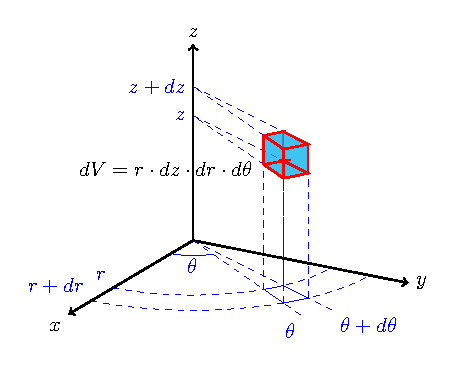
\includegraphics[width=0.5\linewidth]{figure/fig1.4}
	\caption[柱坐标体积元]{柱坐标体积元}
	\label{fig:1.4}
\end{figure}

\begin{example}{柱坐标中自然基底、单位基底与分量的区别}{1,2}
设柱坐标为 $(\rho,\varphi,z)$, 向量场写成自然基底展开: 
\[
\bm{A}
=
\rho^{2}\bm{e}_{\rho}
+
\sin{\varphi}\,\bm{e}_{\varphi}
+
z\bm{e}_{z}.
\]
求 $\bm{A}$ 的逆变分量、协变分量和单位基底下的物理分量. 
\end{example}
\begin{solution}
题目已经将 $\bm{A}$ 写成自然基底展开: 
\[
\bm{A}
=
A^{\rho}\bm{e}_{\rho}
+
A^{\varphi}\bm{e}_{\varphi}
+
A^{z}\bm{e}_{z},
\]
因此逆变分量为
\[
A^{\rho}=\rho^{2},
\qquad
A^{\varphi}=\sin{\varphi},
\qquad
A^{z}=z.
\]
柱坐标的度规由\eqref{eq:1.20}给出, 协变分量由 $A_{i}=g_{ij}A^{j}$ 确定: 
\[
A_{\rho}=g_{\rho\rho}A^{\rho}=\rho^{2},
\qquad
A_{\varphi}=g_{\varphi\varphi}A^{\varphi}
=
\rho^{2}\sin{\varphi},
\qquad
A_{z}=g_{zz}A^{z}=z.
\]
另一方面, 柱坐标的单位基底满足
\[
\hat{\bm{e}}_{\rho}=\bm{e}_{\rho},
\qquad
\hat{\bm{e}}_{\varphi}=\frac{1}{\rho}\bm{e}_{\varphi},
\qquad
\hat{\bm{e}}_{z}=\bm{e}_{z},
\]
即 $\bm{e}_{\varphi}=\rho\hat{\bm{e}}_{\varphi}$, 于是
\[
\bm{A}
=
\rho^{2}\hat{\bm{e}}_{\rho}
+
\rho\sin{\varphi}\,\hat{\bm{e}}_{\varphi}
+
z\hat{\bm{e}}_{z}.
\]
因此物理分量为
\[
A_{\hat{\rho}}=\rho^{2},
\qquad
A_{\hat{\varphi}}=\rho\sin{\varphi},
\qquad
A_{\hat{z}}=z.
\]
该例表明, 在曲线坐标中一般有 $A^{\varphi}\neq A_{\varphi}\neq A_{\hat{\varphi}}$. 
\end{solution}

\begin{example}{由度规推出柱坐标中的拉普拉斯算子}{1,3}
利用一般公式\eqref{eq:1.13}推导柱坐标中的标量拉普拉斯算子. 
\end{example}

\begin{solution}
柱坐标中 $(q^{1},q^{2},q^{3})=(\rho,\varphi,z)$, 度规为\eqref{eq:1.20}, 因此
\[
g=\det{(g_{ij})}=\rho^{2},
\qquad
\sqrt{g}=\rho.
\]
逆变度规为
\[
(g^{ij})
=
\begin{pmatrix}
1&0&0\\
0&\dfrac{1}{\rho^{2}}&0\\
0&0&1
\end{pmatrix}.
\]
代入\eqref{eq:1.13}得
\[
\nabla^{2} f
=
\frac{1}{\rho}
\left[
\partial_{\rho}
\left(
\rho g^{\rho\rho}\partial_{\rho} f
\right)
+
\partial_{\varphi}
\left(
\rho g^{\varphi\varphi}\partial_{\varphi} f
\right)
+
\partial_{z}
\left(
\rho g^{zz}\partial_{z} f
\right)
\right].
\]
由于 $g^{\rho\rho}=1$, $g^{\varphi\varphi}=1/\rho^{2}$, $g^{zz}=1$, 上式化为
\[
\nabla^{2} f
=
\frac{1}{\rho}
\left[
\partial_{\rho}
\left(
\rho\partial_{\rho} f
\right)
+
\partial_{\varphi}
\left(
\frac{1}{\rho}\partial_{\varphi} f
\right)
+
\partial_{z}
\left(
\rho\partial_{z} f
\right)
\right].
\]
由于 $\rho$ 与 $\varphi,z$ 无关, 进一步化简得
\[
\nabla^{2} f
=
\frac{1}{\rho}
\frac{\partial}{\partial\rho}
\left(
\rho\frac{\partial f}{\partial\rho}
\right)
+
\frac{1}{\rho^{2}}
\frac{\partial^{2} f}{\partial\varphi^{2}}
+
\frac{\partial^{2} f}{\partial z^{2}}.
\]
这正是柱坐标中的标量拉普拉斯算子\eqref{eq:1.22}. 
\end{solution}

\section{球坐标}

球坐标记为 $(q^{1},q^{2},q^{3})=(r,\theta,\varphi)$, 其中 $r$ 为径向距离, $\theta$ 为极角, $\varphi$ 为方位角. 
\begin{figure}[h]
	\centering
	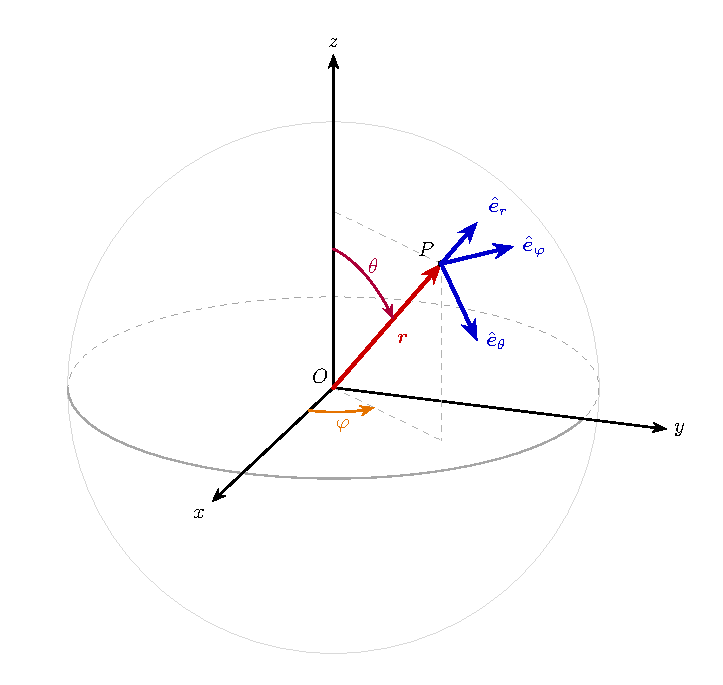
\includegraphics[width=0.5\linewidth]{figure/fig1.3}
	\caption[球坐标系]{球坐标系}
	\label{fig:1.3}
\end{figure}

其位置矢量为
\[
\bm{r}
=
r\sin{\theta}\cos{\varphi}\,\bm{i}
+
r\sin{\theta}\sin{\varphi}\,\bm{j}
+
r\cos{\theta}\,\bm{k}.
\]
自然基底为
\[
\begin{aligned}
	\bm{e}_{r}
	&=
	\frac{\partial\bm{r}}{\partial r}
	=
	\sin{\theta}\cos{\varphi}\,\bm{i}
	+
	\sin{\theta}\sin{\varphi}\,\bm{j}
	+
	\cos{\theta}\,\bm{k},\\
	\bm{e}_{\theta}
	&=
	\frac{\partial\bm{r}}{\partial\theta}
	=
	r\cos{\theta}\cos{\varphi}\,\bm{i}
	+
	r\cos{\theta}\sin{\varphi}\,\bm{j}
	-
	r\sin{\theta}\,\bm{k},\\
	\bm{e}_{\varphi}
	&=
	\frac{\partial\bm{r}}{\partial\varphi}
	=
	-r\sin{\theta}\sin{\varphi}\,\bm{i}
	+
	r\sin{\theta}\cos{\varphi}\,\bm{j}.
\end{aligned}
\]
相应的 Lamé 系数为 $h_{r}=1$, $h_{\theta}=r$, $h_{\varphi}=r\sin{\theta}$, 度规为
\begin{equation}
(g_{ij})
=
\begin{pmatrix}
1&0&0\\
0&r^{2}&0\\
0&0&r^{2}\sin^{2}{\theta}
\end{pmatrix}. \label{eq:1.23}
\end{equation}
线元为
\[
\dif s^{2}
=
(\dif r)^{2}+r^{2}(\dif\theta)^{2}+r^{2}\sin^{2}{\theta}\,(\dif\varphi)^{2}.
\]
体积元为
\[
\dif V
=
r^{2}\sin{\theta}\,\dif r\,\dif\theta\,\dif\varphi.
\]
若 $\bm{A} = A_{\hat{r}}\hat{\bm{e}}_{r} + A_{\hat{\theta}}\hat{\bm{e}}_{\theta} + A_{\hat{\varphi}}\hat{\bm{e}}_{\varphi}$, 则散度为
\begin{equation}
\nabla\cdot\bm{A}
=
\frac{1}{r^{2}}
\frac{\partial}{\partial r}
(r^{2}A_{\hat{r}})
+
\frac{1}{r\sin{\theta}}
\frac{\partial}{\partial\theta}
(\sin{\theta} A_{\hat{\theta}})
+
\frac{1}{r\sin{\theta}}
\frac{\partial A_{\hat{\varphi}}}{\partial\varphi}. \label{eq:1.24}
\end{equation}
标量场 $f$ 的拉普拉斯算子为
\begin{equation}
\nabla^{2} f
=
\frac{1}{r^{2}}
\frac{\partial}{\partial r}
\left(
r^{2}\frac{\partial f}{\partial r}
\right)
+
\frac{1}{r^{2}\sin{\theta}}
\frac{\partial}{\partial\theta}
\left(
\sin{\theta}\frac{\partial f}{\partial\theta}
\right)
+
\frac{1}{r^{2}\sin^{2}{\theta}}
\frac{\partial^{2} f}{\partial\varphi^{2}}. \label{eq:1.25}
\end{equation}
\begin{figure}[h]
	\centering
	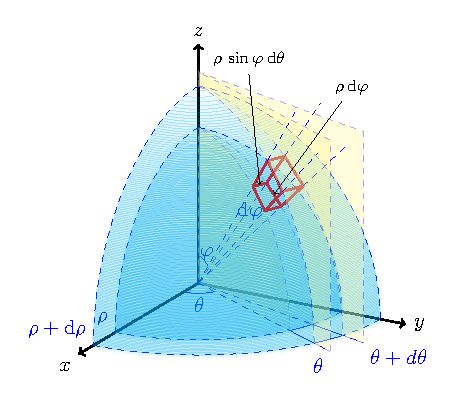
\includegraphics[width=0.5\linewidth]{figure/fig1.5}
	\caption[球坐标体积元]{球坐标体积元}
	\label{fig:1.5}
\end{figure}

\begin{example}{球坐标中径向函数的拉普拉斯算子}{1,4}
设标量场只依赖径向坐标: $f=f(r)$. 求球坐标下的 $\nabla^{2} f$. 
\end{example}

\begin{solution}
球坐标中的标量拉普拉斯算子为\eqref{eq:1.25}. 由于 $f=f(r)$, 角向导数为零, 因此
\[
\nabla^{2} f
=
\frac{1}{r^{2}}
\frac{\dif}{\dif r}
\left(
r^{2}\frac{\dif f}{\dif r}
\right)
=
\frac{\dif^{2} f}{\dif r^{2}}
+
\frac{2}{r}\frac{\dif f}{\dif r}.
\]
特别地, 若 $f(r)=1/r$ ($r\neq 0$), 则 $\dif f/\dif r = -1/r^{2}$, $r^{2}\dif f/\dif r = -1$, 从而
\[
\nabla^{2}\left(\frac{1}{r}\right)
=
\frac{1}{r^{2}}\frac{\dif}{\dif r}(-1)=0,
\qquad r\neq 0.
\]
因此 $1/r$ 在除原点以外的区域是调和函数. 
\end{solution}

\begin{example}{球坐标中点源型径向场的散度}{1,5}
设向量场为 $\bm{A} = \frac{C}{r^{2}}\hat{\bm{e}}_{r}$, 其中 $C$ 为常数. 求 $r\neq 0$ 区域中的 $\nabla\cdot\bm{A}$. 
\end{example}

\begin{solution}
物理分量为 $A_{\hat{r}}=C/r^{2}$, $A_{\hat{\theta}}=0$, $A_{\hat{\varphi}}=0$. 由球坐标散度公式\eqref{eq:1.24}可得
\[
\nabla\cdot\bm{A}
=
\frac{1}{r^{2}}
\frac{\partial}{\partial r}
\left(
r^{2}\frac{C}{r^{2}}
\right)
=
\frac{1}{r^{2}}\frac{\partial C}{\partial r}
=
0,
\qquad r\neq 0.
\]
由此可见在除原点以外的区域, 该场没有普通意义下的散度. 若将原点也包括进来, 则该场在分布意义下满足
\[
\nabla\cdot\left(\frac{C}{r^{2}}\hat{\bm{e}}_{r}\right)
=
4\pi C\,\delta^{(3)}(\bm{r}).
\]
这正是点源场的典型结构. 
\end{solution}

\begin{example}{计算球坐标中的梯度}{1,6}
设标量场 $f(r,\theta,\varphi)=r^{2}\sin{\theta}\cos{\varphi}$, 求 $\nabla f$. 
\end{example}

\begin{solution}
球坐标中 $h_{r}=1$, $h_{\theta}=r$, $h_{\varphi}=r\sin{\theta}$. 由正交曲线坐标梯度公式\eqref{eq:1.16}, 
\[
\nabla f
=
\frac{\partial f}{\partial r}\hat{\bm{e}}_{r}
+
\frac{1}{r}\frac{\partial f}{\partial\theta}\hat{\bm{e}}_{\theta}
+
\frac{1}{r\sin{\theta}}\frac{\partial f}{\partial\varphi}\hat{\bm{e}}_{\varphi}.
\]
各偏导数为
\[
\frac{\partial f}{\partial r} = 2r\sin{\theta}\cos{\varphi},\quad
\frac{\partial f}{\partial\theta} = r^{2}\cos{\theta}\cos{\varphi},\quad
\frac{\partial f}{\partial\varphi} = -r^{2}\sin{\theta}\sin{\varphi}.
\]
因此
\[
\nabla f
=
2r\sin{\theta}\cos{\varphi}\,\hat{\bm{e}}_{r}
+
r\cos{\theta}\cos{\varphi}\,\hat{\bm{e}}_{\theta}
-
r\sin{\varphi}\,\hat{\bm{e}}_{\varphi}.
\]
这是单位基底下的物理分量形式. 若改写为自然基底形式, 利用 $\hat{\bm{e}}_{r}=\bm{e}_{r}$, $\hat{\bm{e}}_{\theta}=\frac{1}{r}\bm{e}_{\theta}$, $\hat{\bm{e}}_{\varphi}=\frac{1}{r\sin{\theta}}\bm{e}_{\varphi}$, 可得
\[
\nabla f
=
2r\sin{\theta}\cos{\varphi}\,\bm{e}_{r}
+
\cos{\theta}\cos{\varphi}\,\bm{e}_{\theta}
-
\frac{\sin{\varphi}}{\sin{\theta}}\bm{e}_{\varphi},
\]
这再次体现了物理分量与逆变分量的区别. 
\end{solution}

\section{本章小结}

本章的核心在于区分曲线坐标的坐标值、向量的张量分量以及单位基底下的物理分量. 

曲线坐标 $q^{i}$ 是点的位置参数, 而不是任意向量的分量. 自然基底由 $\bm{e}_{i} = \frac{\partial\bm{r}}{\partial q^{i}}$ 定义, 逆变基底 $\bm{e}^{i}$ 与之满足 $\bm{e}_{i}\cdot\bm{e}^{j}=\delta_{i}^{j}$. 任意向量可写成 $\bm{A}=A^{i}\bm{e}_{i}=A_{i}\bm{e}^{i}$. 

度规张量 $g_{ij}=\bm{e}_{i}\cdot\bm{e}_{j}$ 决定长度、夹角和指标升降. 在一般曲线坐标中, 散度、旋度和拉普拉斯算子应包含度规或体积因子, 不能直接照搬笛卡尔坐标中的形式. 

在正交曲线坐标中, 还应区分张量分量 $A^{i},A_{i}$ 与物理分量 $A_{\hat{i}}$. 物理教材中常用的柱坐标、球坐标分量通常是单位基底下的物理分量, 而不是张量公式中的协变或逆变分量. 
